%!TEX root = ./main.tex

\section{Experiments} \label{sec:exp}

In this section we include the experiments of the first algorithm for problems with a linear objective function.

\textbf{Implementation.} The first step of our first proposed algorithm is to solve a convex program. In the experiments, we approximate the optimal solution of this program using a vanilla Frank-Wolfe implementation. The linear minimization step within Frank-Wolfe is solved with the Gurobi optimizer.

\textbf{Comparison.} The best standard online algorithm for general covering problems without experts is the online multiplicative weight update (MWU) algorithm. In the experiments we compare our algorithm with the MWU algorithm. When a new constraint arrives in the online problem, the MWU algorithm increases each variable $x_i$ in the constraint with a rate of $\frac{a^t_i}{c_i}(x_i + 1/n)$, where $n$ is the total number of variables. We also compare our results with the optimum offline solution (that knows the whole instance in advance) and the average solution of the experts.
%On the following figures, we display both the first and the second layer execution results of our algorithm (see \cref{fig:my_label}).

\textbf{Input.} First, we evaluated the result of our algorithm on the pathological input of the MWU algorithm. This instance includes $n$ variables and $n$ constraints with uniform costs and coefficients. Each arriving constraint in this pathological example includes one less variable. While the optimal solution is $1$, the worst-case guarantee of MWU is $O(\log n)$. For our algorithm we provided $n$ experts, where $(n-1)$ experts suggest an adversarial trivial solution to set all variables to $1$, while $1$ expert suggests the optimal offline solution. The result of this experiment is visible on \cref{fig:exp-objective}. An important highlight: our algorithm managed to identify the good expert among the majority of adversaries, obtaining a better objective value, than MWU. Second, we experimented with the counter example (in Appendix~\ref{sec:counter-example}) which shows that the claim of \cite{AnandGe22:Online-Algorithms} is unfortunately too strong. The result is also visible on \cref{fig:exp-objective}. Finally, we generated some instances to observe the performance of our algorithm on non-specific inputs.
The specification for the instance generation includes several parameters, which we detail on \cref{fig:exp-params}. The non-specific instances try to represent instances with different 'shape', meaning that the ratio of the number of constraints and variables varies.

To further investigate the impact of the number of variables and the number of experts on our algorithm, we executed the worst case example for the MWU with several input sizes. The result is visible on \cref{fig:exp-3d}.

\textbf{Result.} Multiplicative weight update is a simple and well-performing algorithm in practice. On its pathological worst-case example, our algorithm performs better, however on most instances the expert suggestions were significantly worse than MWU, which impacted the performance of our algorithm. To some extent, our algorithm can detect the good experts and is robust against even many adversaries. We think that given a real-life problem, it is possible to construct well-performing experts (for example using past data) and with a fine-tuned convex program solver our algorithm can be of interest for various use-cases.

\begin{figure}[!ht]
\centering
\begin{tabular}{r|r|r|r|r|r|r}
          & Worst-case & Counter-ex. & & & & \\
Algo name & for MWU  & for \cite{AnandGe22:Online-Algorithms} & Inst. $1$ & Inst. $2$ & Inst. $3$ & Inst. $4$\\
\hline
OPT Offline            & 1.0 & 1.0 & 1.3 & 1.5 & 10.6 & 31.3 \\
MWU Online             & 2.9 & 2.3 & 2.0 & 1.7 & 28.1 & 63.7 \\
\hline
%Our Algo               & 1.6 & 5.8 & 24.5 & \textbf{17.5}\\
Our Algo           & {\bf 2.2} & {\bf 4.4} & {\bf 2.0} & {\bf 1.7} & {\bf 26.7}  & {\bf 61.7} \\
\hline
Avg of experts      & 9.1 & 3.5 & 16.4 & 23.3 & 1897.47 & 96.9 \\
\end{tabular}
\caption{Objective value of the experiment instances}
\label{fig:exp-objective}
\end{figure}

\begin{figure}[!ht]
\centering
\begin{tabular}{l|r|r|r|r}
Input Generation Parameters & Instance $1$ & Instance $2$ & Instance $3$ & Instance $4$ \\
\hline
Number of variables            & 10 & 10 & 44  & 30 \\
Number of constraints          & 10 & 25 & 2   & 15 \\
Min objective coefficient      & 1  & 10 & 1   & 1  \\
Max objective coefficient      & 10 & 25 & 100 & 100\\
Min constraint coefficient     & 1  & 10 & 1   & 1 \\
Max constraint coefficient     & 10 & 25 & 1   & 1 \\
Min number of zero coefficient & 0  &  1 & 11  & 5 \\
Max number of zero coefficient & 5  &  5 & 22  & 20 \\
Number of perfect experts      & 1  &  0 & 0   & 2 \\
Number of online experts       & 2  &  1 & 1   & 2 \\
Number of random experts       & 1  &  1 & 11  & 0 \\
Number of adversaries          & 1  &  1 & 0   & 0 \\
\end{tabular}
\caption{Parameters of the generated experiment instances}
\label{fig:exp-params}
\end{figure}

\begin{figure}[!ht]
    \centering
    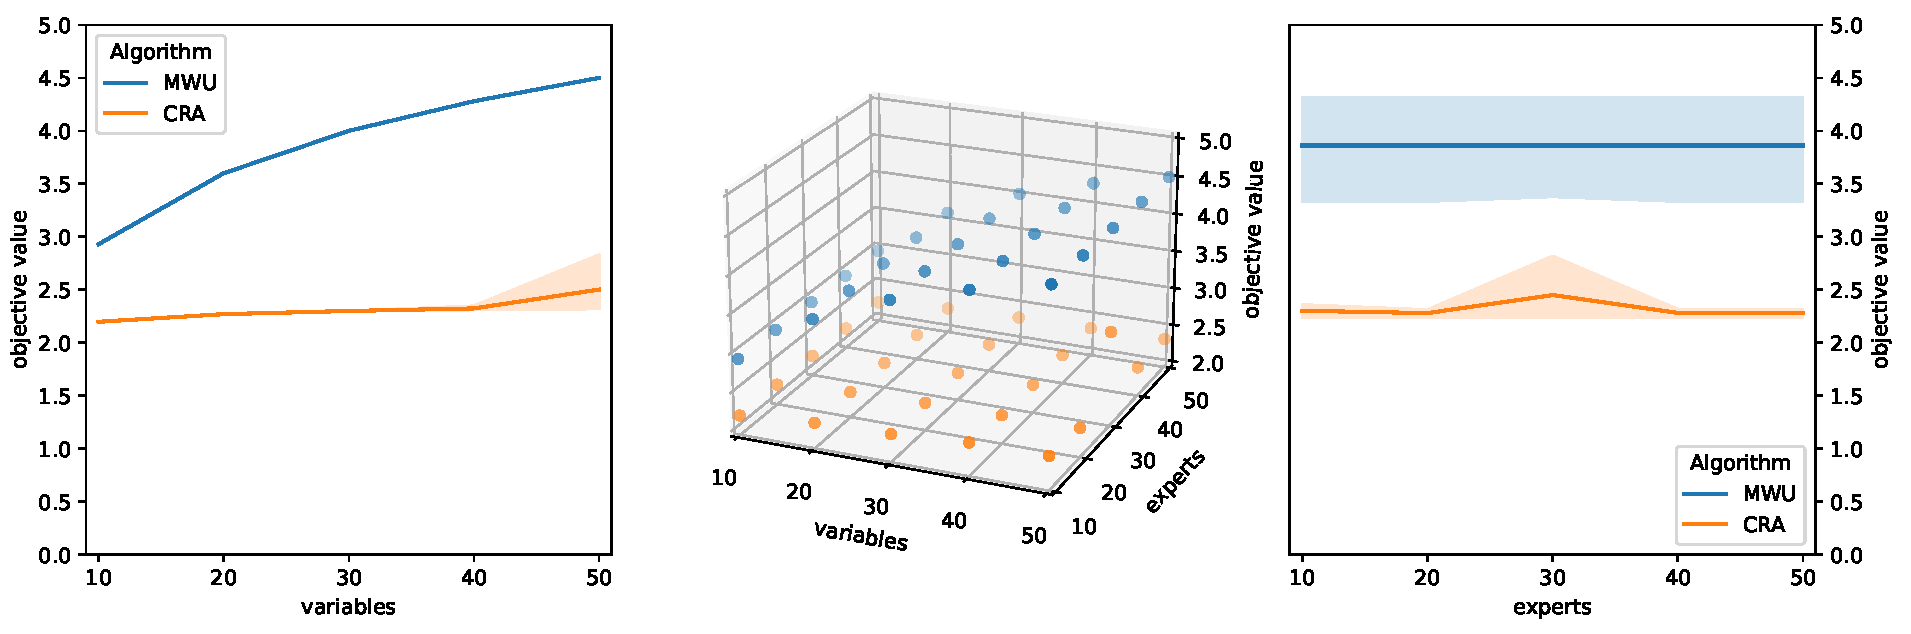
\includegraphics[width=\linewidth]{Img/worst_case_figure.pdf}
    \caption{Experiment with varying number of variables and experts on the MWU worst-case instance}
    \label{fig:exp-3d}
\end{figure}